\documentclass[11pt]{article}

\usepackage{graphicx}
\usepackage{hyperref}
\usepackage{natbib}
\usepackage{amsmath}

\bibliographystyle{plain}
\setlength{\textwidth}{6.5in}
\setlength{\headheight}{0in}
\setlength{\textheight}{8.0in}
\setlength{\hoffset}{0in}
\setlength{\voffset}{0in}
\setlength{\oddsidemargin}{0in}
\setlength{\evensidemargin}{0in}


\title{Computational Physics -  Problem Set 10}
  
\author{Frederik Holst Knudsen}


\begin{document}

\maketitle
Github URL: https://github.com/frederikholst/phys-ga2000
\section{Newman 9.8}
We use the Crank Nicolson method to time evolve the wavefunction of an electron in an infinite square well. See Figure \ref{one} for the first step with temporal step size $h=1\times 10^{-18}s$, spatial step size $a=L/N$ where $L=1\times 10^{-8}m$ and $N=1000$ is length of the square well and the number spatial points respectively. To compute the wavefunction at times $t+h$, we solve for x using the Crank Nicolson method: 
\begin{equation}
\mathbf{A}\psi(t+h)=\mathbf{B}\psi(t)
\end{equation}

where the solution of $\psi(t+h)$ is found using the banded matrix solver from Newman's Online Resources. 

\begin{figure}[!htbp]
    \centering
    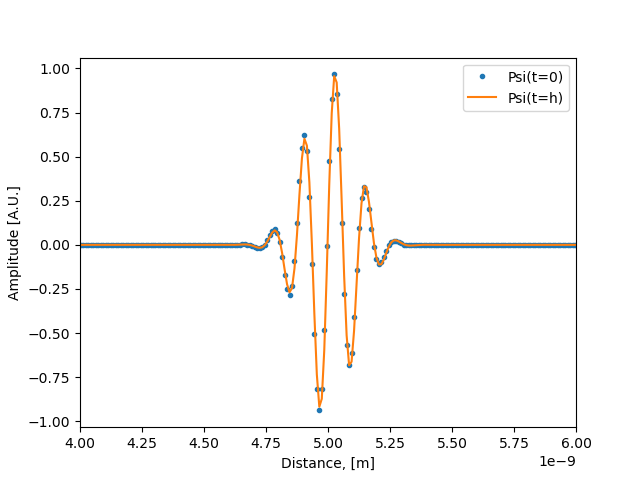
\includegraphics[width=0.7\textwidth]{One Step.png}
    \caption{The first step of the real part of the wavefunction after a very small time step, h. We see that the first step almost entirely overlaps the initial wavepacket.}
    \label{one}
\end{figure}

We then proceed and calculate many more time steps to capture the dynamics of the system. See Figure \ref{ten} for ten wavefunctions at different times.
\begin{figure}[!htbp]
    \centering
    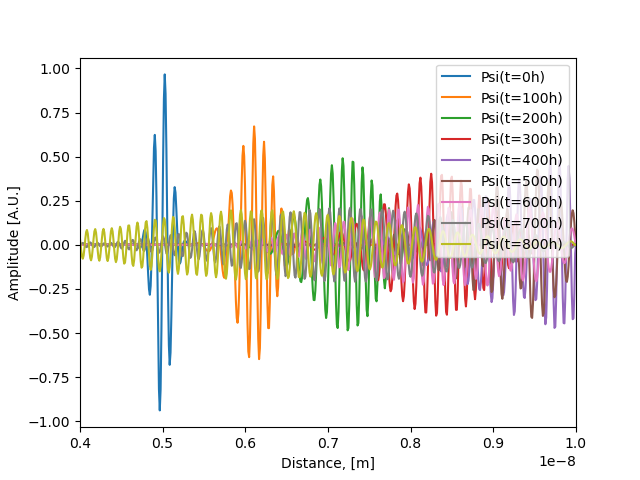
\includegraphics[width=0.7\textwidth]{10 waves.png}
    \caption{The dynamics of the real part of the wavepacket moving to the right at later and later time steps, with $h=1\times 10^{-18}s$ is the size of one time step. We also clearly see effects of broadening and scattering as it hits the wall of the potential.}
    \label{ten}
\end{figure}

Finally we set up the first 2000 time steps in matplotlib's animation package and produce an animation of the scattering of the electron off the right wall of the potential. One might think this looks like a propagating audio wave, but this is indeed an electron moving to the right with larger and larger broadening. When it hits the potential barrier, it picks up some higher oscillating terms and becomes increasingly my disonant. The electron then bounces off the wall and scatters to the left. This hints at the large complexity of finding analytic solutions to scattering problems. 


\section{Newman 9.9}

We now turn to solve the Schrödinger equation using the spectral method. We do this by making a Fourier transform of the initial wavepacket and insert the real and imaginary fourier coefficients in the formular as discribed in Newman. See Figure \ref{spectral} for the plotted solution to the Schrödinger equation at an advanced time. 

\begin{figure}[!htbp]
    \centering
    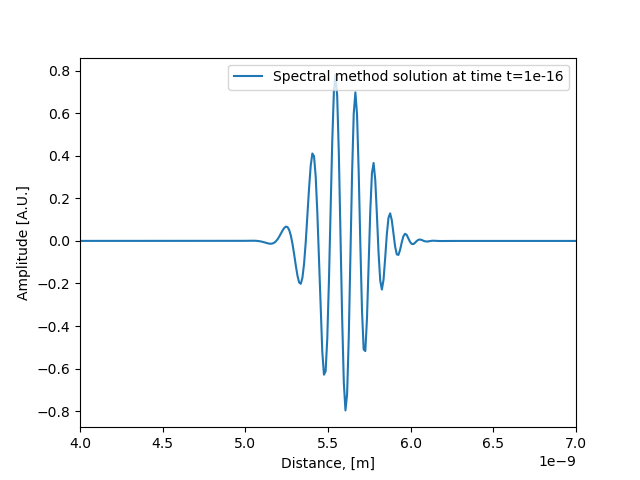
\includegraphics[width=0.7\textwidth]{Spectral Method.png}
    \caption{The Schrödinger equation solved at t=1e-16s using the spectral method for an electon in an infinite square well. We see strong agreement with that of the previous problem using the Crank-Nielson finite step method.}
    \label{spectral}

It is now possible for us to make a series of solutions to the Schrödinger equation at different times and compose an animation of these using the matplotlib animation package as before. Physically this represents the same scenario, with the electron represented as the real part of a wavefunction that scatters off the side of the potential barrier and starts to propagate in the other direction. 
\end{figure}
\end{document}


\begin{figure}[!htbp]
    \centering
    \includegraphics[width=0.7\textwidth]{.png}
    \caption{}
    \label{v}
\end{figure}
